\section{\LaTeX~Beispiele}

\subsection{Zitieren}
Das Projektmanagement orientiert sich an Bruno Jenny \cite{jenny} und einigen anderen Aspekten \cite{wiki:projektmanagement}.

\subsection{Grafiken}
Grafiken werden mittels einer einfachen Umgebung eingebettet. Diese können entweder einfach sein oder gemischt.

\begin{figure}[h!]\label{federpendel}
	\centering
	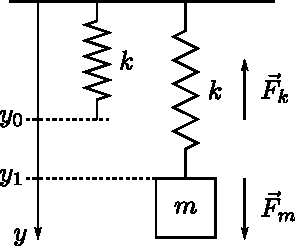
\includegraphics[scale=0.5]{federpendel-vertikal.pdf}
	\caption{Federpendel}
\end{figure}

Wie auf alle anderen Inhalte können auch bei Grafiken Referenzen gesetzt
werden, auf die von überall her hin referenziert werden kann. Dies geht 
auch bei kombinierten Grafiken. Die Grafik \ref{fig:federanordnung} zeigt
zwei geläufige Federanordnungen, wobei die Grafik \ref{fig:serielle_feder}
eine serielle Federanordnung zeigt und \ref{fig:parallele_feder} eine
parallele Anordnung.

\begin{figure}[h!]
        \centering
        \begin{subfigure}[c]{0.4\textwidth}
		\centering
                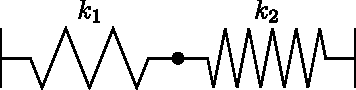
\includegraphics[width=\textwidth]{feder-seriell.pdf}
                \caption{Serielle Federanordnung}
                \label{fig:serielle_feder}
        \end{subfigure}%
        \begin{subfigure}[c]{0.4\textwidth}
		\centering
                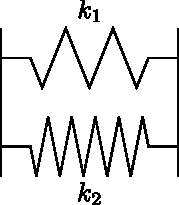
\includegraphics[width=0.4\textwidth]{feder-parallel.pdf}
                \caption{Parallele Federanordnung}
                \label{fig:parallele_feder}
        \end{subfigure}
        \caption{Federanordnungen}\label{fig:federanordnung}
\end{figure}
